\chapter{Potential Energy Landscapes, Equilibrium, and Stability}
\label{ch:stability_wells}

\begin{chapterintro}
\textbf{Chapter Objectives:} In this chapter, we develop the geometric and analytical theory of one-dimensional potential energy landscapes. You will learn to identify classically allowed regions and turning points; systematically classify points of equilibrium as stable, unstable, or neutral; calculate effective stiffness coefficients $k_{\text{eff}} = E_p''(x_0)$ via Taylor expansions; compute natural frequencies of small oscillations; and analyze canonical potentials including the Lennard-Jones (6-12) molecular potential and the quartic double-well.
\end{chapterintro}

\section{One-Dimensional Potential Landscapes and Turning Points}

Consider a material point of mass $m$ constrained to move along the $x$-axis under the action of a conservative force $F(x) = -\frac{\dd E_p}{\dd x}$. By the conservation of mechanical energy:
\begin{equation}
E_m = \frac{1}{2}m \dot{x}^2 + E_p(x) = \text{constant}.
\end{equation}
Because kinetic energy is intrinsically non-negative ($E_k = \frac{1}{2}m\dot{x}^2 \ge 0$), the particle can only exist in spatial regions where the total mechanical energy equals or exceeds the potential energy:
\begin{equation}
E_p(x) \le E_m.
\end{equation}

\begin{figure}[htbp]
\centering
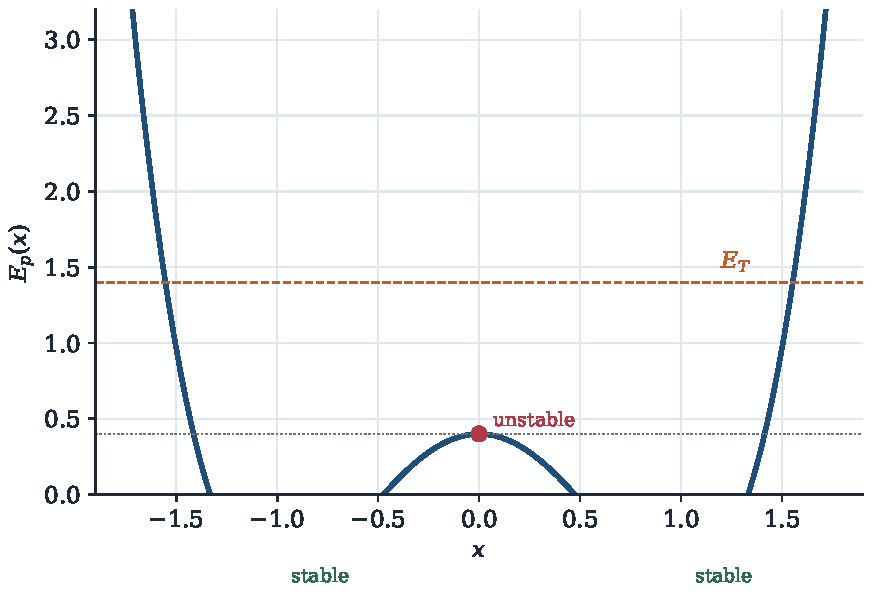
\includegraphics[width=0.74\textwidth]{figures/15_energy_well.pdf}
\caption{One-dimensional potential energy landscape $E_p(x)$. For a particle with mechanical energy $E_m$, the motion is confined to the classically allowed region between the turning points $x_1$ and $x_2$ where $E_p(x) = E_m$. At local minima ($x_0$), equilibrium is stable; at local maxima ($x_{\text{max}}$), equilibrium is unstable.}
\label{fig:energy_well}
\end{figure}

Solving the energy conservation equation for the velocity $\dot{x} = \dd x/\dd t$:
\begin{equation}
\dot{x} = \pm \sqrt{\frac{2}{m}\left( E_m - E_p(x) \right)}.
\end{equation}

\begin{definitionbox}{Classically Allowed Regions and Turning Points}
\begin{itemize}[leftmargin=1.5em,itemsep=3pt]
  \item \textbf{Classically Allowed Region:} The set of coordinates $\{x \in \mathbb{R} \mid E_p(x) \le E_m\}$. The kinetic energy is positive, and the particle moves with real non-zero velocity.
  \item \textbf{Classically Forbidden Region:} The set of coordinates $\{x \in \mathbb{R} \mid E_p(x) > E_m\}$. In classical mechanics, penetration into this region is strictly impossible because it would require imaginary velocity (or negative kinetic energy).
  \item \textbf{Turning Points (Inversion Points):} The spatial boundaries $x_t$ where the mechanical energy line intersects the potential curve:
  \begin{equation}
  E_p(x_t) = E_m \implies v(x_t) = 0.
  \end{equation}
  At a turning point, the particle comes to rest instantaneously, reverses its direction of motion, and accelerates back into the well under the force $F(x_t) = -E_p'(x_t)$.
\end{itemize}
\end{definitionbox}

If the allowed region is a finite interval $[x_1, x_2]$ bounded by two turning points ($E_p(x_1) = E_p(x_2) = E_m$), the particle is trapped in a \textbf{potential well} and executes bounded periodic oscillatory motion. The exact period of oscillation $T$ is given by separating variables $\dd t = \frac{\dd x}{\sqrt{\frac{2}{m}(E_m - E_p(x))}}$:
\begin{equation}
T = 2 \int_{x_1}^{x_2} \frac{\dd x}{\sqrt{\frac{2}{m}\left( E_m - E_p(x) \right)}}.
\end{equation}

\section{Equilibrium Points and Stability Classification}

A material point is in mechanical equilibrium if the net force acting on it vanishes:
\begin{equation}
F(x_0) = 0 \iff \left.\frac{\dd E_p}{\dd x}\right|_{x_0} = 0.
\end{equation}
Thus, \textbf{the points of equilibrium correspond geometrically to the stationary points (horizontal tangents) of the potential energy curve}.

To evaluate the stability of an equilibrium point $x_0$, we perform a Taylor series expansion of the potential energy $E_p(x)$ around $x_0$ for small displacements $\eta \eqdef x - x_0$:
\begin{equation}
E_p(x_0 + \eta) = E_p(x_0) + \underbrace{\left.\frac{\dd E_p}{\dd x}\right|_{x_0}}_{= 0}\eta + \frac{1}{2}\left.\frac{\dd^2 E_p}{\dd x^2}\right|_{x_0}\eta^2 + \frac{1}{6}\left.\frac{\dd^3 E_p}{\dd x^3}\right|_{x_0}\eta^3 + \mathcal{O}(\eta^4).
\end{equation}
Defining the \textbf{effective spring constant}:
\begin{equation}
k_{\text{eff}} \eqdef \left.\frac{\dd^2 E_p}{\dd x^2}\right|_{x_0}.
\end{equation}
The restoring force acting on the displaced particle is:
\begin{equation}
F(\eta) = -\frac{\dd E_p}{\dd\eta} \approx -k_{\text{eff}}\,\eta - \frac{1}{2} E_p'''(x_0)\,\eta^2.
\end{equation}

\begin{lawbox}{Classification of Equilibrium States}
\begin{enumerate}[leftmargin=1.5em,itemsep=4pt]
  \item \textbf{Stable Equilibrium ($k_{\text{eff}} > 0$):}
  The potential energy curve is concave upward ($\frac{\dd^2 E_p}{\dd x^2} > 0$), possessing a \textbf{local minimum} at $x_0$. A positive displacement ($\eta > 0$) induces a negative restoring force ($F < 0$), pulling the particle back toward $x_0$.
  \item \textbf{Unstable Equilibrium ($k_{\text{eff}} < 0$):}
  The potential energy curve is concave downward ($\frac{\dd^2 E_p}{\dd x^2} < 0$), possessing a \textbf{local maximum} at $x_0$. Any infinitesimal displacement ($\eta \neq 0$) produces a repulsive force ($F \approx |k_{\text{eff}}|\eta$) accelerating the particle away from $x_0$ exponentially: $\eta(t) \propto e^{\lambda t}$ with $\lambda = \sqrt{|k_{\text{eff}}|/m}$.
  \item \textbf{Neutral (Indifferent) Equilibrium ($k_{\text{eff}} = 0$):}
  The potential is locally flat to second order. Stability is determined by the first non-vanishing higher derivative $E_p^{(n)}(x_0)$:
  \begin{itemize}[leftmargin=1.2em,itemsep=2pt]
    \item If $n$ is odd, the point is an inflection point and is \emph{unstable}.
    \item If $n$ is even and $E_p^{(n)}(x_0) > 0$, the equilibrium is \emph{stable}.
    \item If $n$ is even and $E_p^{(n)}(x_0) < 0$, the equilibrium is \emph{unstable}.
  \end{itemize}
\end{enumerate}
\end{lawbox}

\begin{figure}[htbp]
\centering
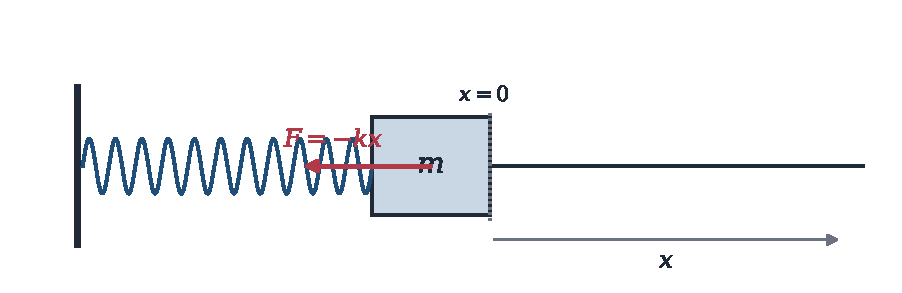
\includegraphics[width=0.62\textwidth]{figures/14_spring_mass.pdf}
\caption{The universal harmonic prototype: a mass-spring system whose quadratic potential $E_p(x) = \frac{1}{2}k x^2$ models the bottom of any generic smooth potential energy well.}
\label{fig:spring_mass}
\end{figure}

\section{The Harmonic Approximation and Small Oscillations}

Near any regular stable equilibrium minimum $x_0$ ($k_{\text{eff}} = E_p''(x_0) > 0$), we truncate the Taylor expansion at quadratic order:
\begin{equation}
E_p(\eta) \approx E_p(x_0) + \frac{1}{2} k_{\text{eff}}\,\eta^2.
\end{equation}
Newton's second law for the displacement $\eta(t) = x(t) - x_0$ yields:
\begin{equation}
m \frac{\dd^2\eta}{\dd t^2} = F(\eta) \approx -k_{\text{eff}}\,\eta \implies \frac{\dd^2\eta}{\dd t^2} + \omega_0^2\,\eta = 0.
\end{equation}

\begin{lawbox}{Universal Frequency of Small Oscillations}
For sufficiently small perturbations about any stable equilibrium point $x_0$, the motion is universally simple harmonic with natural angular frequency:
\begin{equation}
\omega_0 \eqdef \sqrt{\frac{k_{\text{eff}}}{m}} = \sqrt{\frac{1}{m}\left.\frac{\dd^2 E_p}{\dd x^2}\right|_{x_0}}.
\end{equation}
The natural period of small oscillations is:
\begin{equation}
T_0 = \frac{2\pi}{\omega_0} = 2\pi\sqrt{\frac{m}{E_p''(x_0)}}.
\end{equation}
\end{lawbox}

This remarkable theorem implies that \textbf{all physical systems, no matter how complex their underlying microscopic forces, behave as simple harmonic oscillators in the limit of small displacements about a stable equilibrium}.

\section{Comprehensive Worked Examples}

\begin{workedexample}{The Lennard-Jones (6-12) Intermolecular Potential}
The interaction potential between two neutral noble gas atoms (e.g., Argon) separated by a distance $r > 0$ is accurately described by the empirical Lennard-Jones (6-12) potential:
\begin{equation}
V(r) = 4\varepsilon \left[ \left(\frac{\sigma}{r}\right)^{12} - \left(\frac{\sigma}{r}\right)^6 \right],
\end{equation}
where $\varepsilon > 0$ is the depth of the attractive well and $\sigma > 0$ is the distance at which the interatomic potential vanishes ($V(\sigma) = 0$).
\begin{enumerate}[leftmargin=1.4em,itemsep=3pt]
  \item Derive the interatomic interaction force $F(r) = -\frac{\dd V}{\dd r}$ and identify the repulsive and attractive regimes.
  \item Determine the equilibrium separation distance $r_0$ and compute the binding energy $V(r_0)$.
  \item Calculate the effective spring constant $k_{\text{eff}} = V''(r_0)$ and determine the frequency $\omega_0$ of small molecular vibrations for a diatomic molecule of reduced mass $\mu$.
\end{enumerate}

\paragraph{Solution.}
\textbf{1. Interatomic Force:}\\
Differentiating the Lennard-Jones potential with respect to $r$:
\[
F(r) = -\frac{\dd V}{\dd r} = -4\varepsilon \left[ -12\frac{\sigma^{12}}{r^{13}} - \left(-6\frac{\sigma^6}{r^7}\right) \right] = \frac{24\varepsilon}{r}\left[ 2\left(\frac{\sigma}{r}\right)^{12} - \left(\frac{\sigma}{r}\right)^6 \right].
\]
\begin{itemize}[leftmargin=1.5em,itemsep=2pt]
  \item When $r < 2^{1/6}\sigma$, $2(\sigma/r)^{12} > (\sigma/r)^6$, so $F(r) > 0$: the force is strongly \textbf{repulsive}, originating from Pauli exclusion between overlapping electronic clouds.
  \item When $r > 2^{1/6}\sigma$, $2(\sigma/r)^{12} < (\sigma/r)^6$, so $F(r) < 0$: the force is \textbf{attractive}, corresponding to long-range induced dipole-dipole (van der Waals / London dispersion) interactions.
\end{itemize}

\textbf{2. Equilibrium Distance and Well Depth:}\\
Equilibrium occurs where the net force vanishes, $F(r_0) = 0$:
\[
2\left(\frac{\sigma}{r_0}\right)^{12} = \left(\frac{\sigma}{r_0}\right)^6 \implies \left(\frac{\sigma}{r_0}\right)^6 = \frac{1}{2} \implies r_0 = 2^{1/6}\,\sigma \approx 1.12246\,\sigma.
\]
Evaluating the potential at this equilibrium distance:
\[
V(r_0) = 4\varepsilon \left[ \left(\frac{1}{2}\right)^2 - \frac{1}{2} \right] = 4\varepsilon \left( \frac{1}{4} - \frac{1}{2} \right) = 4\varepsilon \left(-\frac{1}{4}\right) = -\varepsilon.
\]
The potential well depth is exactly $-\varepsilon$. A minimum energy $\Delta E = +\varepsilon$ (the dissociation energy) must be supplied to separate the atoms to infinite distance.

\textbf{3. Effective Stiffness and Vibrational Frequency:}\\
Differentiating $F(r)$ to compute the second derivative of the potential:
\[
V''(r) = -\frac{\dd F}{\dd r} = -\frac{\dd}{\dd r}\left( \frac{48\varepsilon \sigma^{12}}{r^{13}} - \frac{24\varepsilon \sigma^6}{r^7} \right) = \frac{48 \times 13\,\varepsilon \sigma^{12}}{r^{14}} - \frac{24 \times 7\,\varepsilon \sigma^6}{r^8}.
\]
Evaluating at $r_0$ where $(\sigma/r_0)^6 = 1/2$ and $(\sigma/r_0)^{12} = 1/4$:
\[
V''(r_0) = \frac{\varepsilon}{r_0^2}\left[ 48 \times 13 \left(\frac{\sigma}{r_0}\right)^{12} - 24 \times 7 \left(\frac{\sigma}{r_0}\right)^6 \right] = \frac{\varepsilon}{r_0^2}\left[ 624\left(\frac{1}{4}\right) - 168\left(\frac{1}{2}\right) \right].
\]
\[
V''(r_0) = \frac{\varepsilon}{r_0^2}\left[ 156 - 84 \right] = \frac{72\,\varepsilon}{r_0^2} = \frac{72\,\varepsilon}{2^{1/3}\sigma^2} \approx \frac{57.14\,\varepsilon}{\sigma^2} > 0.
\]
Since $V''(r_0) > 0$, the equilibrium is strictly stable. The natural vibrational frequency of the diatomic molecule is:
\[
\omega_0 = \sqrt{\frac{k_{\text{eff}}}{\mu}} = \sqrt{\frac{72\varepsilon}{\mu\, r_0^2}} = \frac{6}{r_0}\sqrt{\frac{2\varepsilon}{\mu}},
\]
where $\mu = \frac{m_1 m_2}{m_1 + m_2}$ is the reduced mass of the pair.
\end{workedexample}

\begin{workedexample}{The Quartic Double-Well Potential and Symmetry Breaking}
A particle of mass $m$ moves in a one-dimensional symmetrical quartic potential:
\begin{equation}
E_p(x) = -\frac{1}{2}\alpha\, x^2 + \frac{1}{4}\beta\, x^4, \qquad \alpha > 0,\ \beta > 0.
\end{equation}
\begin{enumerate}[leftmargin=1.4em,itemsep=3pt]
  \item Find all equilibrium positions and classify their stability.
  \item Determine the potential depth at the stable minima and sketch the energy threshold separating oscillatory motion confined to a single well from large-scale oscillations crossing both wells.
  \item Find the frequency $\omega_0$ of small oscillations about the stable minima.
\end{enumerate}

\paragraph{Solution.}
\textbf{1. Equilibrium Points:}\\
The force is $F(x) = -E_p'(x) = \alpha x - \beta x^3 = x(\alpha - \beta x^2)$.
Equilibrium points satisfy $F(x) = 0$:
\[
x_0 = 0, \qquad \text{or} \qquad x_{\pm} = \pm \sqrt{\frac{\alpha}{\beta}}.
\]
To classify their stability, we evaluate the second derivative:
\[
E_p''(x) = -\alpha + 3\beta x^2.
\]
\begin{itemize}[leftmargin=1.5em,itemsep=2pt]
  \item At the origin $x_0 = 0$:
  \[
  E_p''(0) = -\alpha < 0 \implies \textbf{Unstable equilibrium (local maximum)}.
  \]
  \item At the twin equilibria $x_{\pm} = \pm\sqrt{\alpha/\beta}$:
  \[
  E_p''(x_{\pm}) = -\alpha + 3\beta\left(\frac{\alpha}{\beta}\right) = 2\alpha > 0 \implies \textbf{Stable equilibria (twin local minima)}.
  \]
\end{itemize}

\textbf{2. Well Depth and Energy Regimes:}\\
Evaluating the potential at the equilibria:
\[
E_p(0) = 0, \qquad E_p(x_{\pm}) = -\frac{1}{2}\alpha\left(\frac{\alpha}{\beta}\right) + \frac{1}{4}\beta\left(\frac{\alpha}{\beta}\right)^2 = -\frac{\alpha^2}{2\beta} + \frac{\alpha^2}{4\beta} = -\frac{\alpha^2}{4\beta}.
\]
The potential possesses two symmetric minima of depth $-\Delta E = -\frac{\alpha^2}{4\beta}$ separated by a central potential barrier of height $E_p(0) = 0$.
\begin{itemize}[leftmargin=1.5em,itemsep=2pt]
  \item If $-\frac{\alpha^2}{4\beta} < E_m < 0$: the motion is bounded inside either the left well ($x < 0$) or the right well ($x > 0$). The particle cannot cross the barrier at $x = 0$. The reflection symmetry of the system is \emph{spontaneously broken} by the particle's choice of well.
  \item If $E_m = 0$: this is the \textbf{separatrix}. The particle reaches $x = 0$ asymptotically as $t \to \infty$.
  \item If $E_m > 0$: the particle has sufficient energy to surmount the central barrier, executing wide oscillations enclosing both minima between turning points $x = \pm x_t$.
\end{itemize}

\textbf{3. Frequency of Small Oscillations:}\\
Near either stable minimum $x = x_{\pm}$, the effective stiffness is $k_{\text{eff}} = E_p''(x_{\pm}) = 2\alpha$.
The natural angular frequency of small oscillations is:
\[
\omega_0 = \sqrt{\frac{k_{\text{eff}}}{m}} = \sqrt{\frac{2\alpha}{m}}.
\]
This model represents the classic Landau theory of second-order phase transitions, spontaneous symmetry breaking in quantum field theory (the Higgs mechanism), and the inversion vibration of the ammonia molecule ($\mathrm{NH}_3$).
\end{workedexample}

\begin{workedexample}{Vertical Hydrodynamic Stability and Bobbing of a Floating Spar}
A solid vertical cylindrical spar buoy of uniform mass $m$, total length $H$, and constant cross-sectional area $S$ floats vertically in a calm sea of water of density $\rho_w$. The density of the spar is $\rho_s < \rho_w$.
\begin{enumerate}[leftmargin=1.4em,itemsep=3pt]
  \item Determine the equilibrium submerged draft $h_0$.
  \item Express the total potential energy $E_p(z)$ as a function of the vertical displacement $z$ from equilibrium.
  \item Show that the vertical equilibrium is unconditionally stable and compute the period of small vertical heaving oscillations.
\end{enumerate}

\paragraph{Solution.}
\textbf{1. Equilibrium Draft:}\\
Let $h_0$ be the submerged depth in static equilibrium. The buoyant force (Archimedes' principle) equals the weight of displaced fluid:
\[
F_{\text{buoyant}} = \rho_w S h_0\, g.
\]
The gravitational weight of the spar is $P = m g = \rho_s S H\, g$.
Equating buoyancy to weight:
\[
\rho_w S h_0 g = \rho_s S H g \implies h_0 = \frac{\rho_s}{\rho_w} H.
\]

\textbf{2. Potential Energy Function:}\\
Let $z$ be the upward vertical displacement from the equilibrium draft $h_0$. When the cylinder is displaced upward by $z$, its submerged depth becomes $h = h_0 - z$.
The net vertical restoring force acting on the spar is:
\[
F_z(z) = F_{\text{buoyant}} - P = \rho_w S (h_0 - z) g - mg = \rho_w S h_0 g - \rho_w S g z - mg.
\]
Since $\rho_w S h_0 g = mg$:
\[
F_z(z) = -\rho_w S g\, z.
\]
The potential energy associated with this linear restoring force (taking $E_p(0) = 0$ at equilibrium) is:
\[
E_p(z) = -\int_0^z F_z(z')\,\dd z' = \int_0^z \rho_w S g\, z'\,\dd z' = \frac{1}{2} \rho_w S g\, z^2.
\]

\textbf{3. Stability and Heaving Period:}\\
Evaluating the second derivative of the potential energy:
\[
k_{\text{eff}} = \left.\frac{\dd^2 E_p}{\dd z^2}\right|_{z = 0} = \rho_w S g > 0.
\]
Because $\rho_w S g > 0$ strictly, the vertical equilibrium is unconditionally stable.
The differential equation of motion is:
\[
m \ddot{z} + \rho_w S g z = 0 \implies \ddot{z} + \omega_0^2 z = 0, \qquad \omega_0 = \sqrt{\frac{\rho_w S g}{m}}.
\]
Substituting $m = \rho_s S H = \rho_w S h_0$:
\[
\omega_0 = \sqrt{\frac{\rho_w S g}{\rho_w S h_0}} = \sqrt{\frac{g}{h_0}}.
\]
The natural period of vertical heaving oscillations is:
\[
T_0 = \frac{2\pi}{\omega_0} = 2\pi\sqrt{\frac{h_0}{g}}.
\]
This expression is formally identical to the period of a simple pendulum of length $L = h_0$, demonstrating the mathematical unity of classical mechanics.
\end{workedexample}
